\pagebreak
\section{String Enumeration Formulas}\label{sec_sef}

\subsection{Enumeration of infinite binary strings}

Next, we will define \textit{string enumeration formulas} (SEFs) by overloading the round brackets (parentheses) notation to indicate the occurrence of a cyclic string.

Let us revise the notations that we have already reserved to describe binary strings. We want to see in which cases the same can be expressed even shorter. To achieve this we would require such notation to be more compact and yet to denote the same value of the corresponding infinite binary string.

Let us start with the bi-infinite string which has a value of $b$, which can be computed as concatenation of repeating $\bos01\eos$ substrings countably many times, as $b = \bos..010101..\eos$\footnote{We reserve \textit{two sequential dots} or ".." notation to denote omitted range in any assumed infinite binary string, but for other infinite sequences we keep \textit{ellipses} with "..." to mean same}. We will denote such repetitive motif with round brackets. If no finite length index was specified, then such brackets indicate an infinite cycle, s.t. $\bos..0101010101..\eos \backsim \bos(01)\eos$. In other words $\bos(01)\eos$ is a program that can be computed to print out the infinite value it is representing.

\begin{definition}Replicator or replication operator is a simple program denoted by round brackets that repeats the finite substring value wrapped in those brackets countably many times.\end{definition}

\begin{definition}String enumeration formula is a program implementing a second order replicator. Formulas can be nested in each other, so that one formula can contain either other formulas or concatenation of multiple replicators. Each replicator is always a balanced pair of brackets. Any closing bracket must be always preceded by the opening one, so that the whole expression can be parsed as a tree from the infix notation of the formula.\end{definition}

For example, a basic formula contains a single replicator and can be implemented by an infinite printing loop. We also say that two formulas $\bos(01)\eos \neq \bos(10)\eos$ represent different bi-infinite binary strings or are equal modular up to the shift from their initial index position at zero ("in the middle" of each string). Namely, $b=(01): b(-1)= 1, b(0)=0, b(1)=1 , ... , \forall i \in I, I \subset \integers$ and $b^\prime=(10): b^\prime(-1)=0, b^\prime(0)=1, b^\prime(1)=0, ... , \forall i \in I, I \subset \integers$.



\subsection{Categorization of SEFs}

Now let's reiterate the idea of building an infinite binary string without any repetition. For that we will need another shorthand in our notations that we can use as a part of SEFs. We will use square brackets to note conversion of the natural number into binary format\footnote{low-endian and without zero-padding}. Here are a few examples of employing this notation:

\begin{itemize}
  \item $\bos([0])\eos \backsim \bos(0)\eos$
  \item $\bos([1])\eos \backsim \bos(1)\eos$
  \item $\bos([2])\eos \backsim \bos(10)\eos$
  \item $\bos([3])\eos \backsim \bos(11)\eos$
  \item $\bos([4])\eos \backsim \bos(100)\eos$
  \item ...
\end{itemize}

Intuitively, counting can be one of the obvious ways of generating examples of non-cyclic infinite binary strings, i.e. by enumerating natural number sequence in a single line. Following the above notation and adding a plus sign that would mean

\begin{center}$ \bos(0)[1+]\eos \backsim \bos(0)[1][2][3][4][5][6][7][8]..\eos \backsim \bos..00000110111001011101111000..\eos$\end{center}

Although the square brackets notation does not necessarily enrich the expressiveness of SEFs, it is still a useful shortcut for the discussion purposes.

So far we have defined cyclic and non-cyclic infinite binary strings. These are a rather \textit{trivial} but not the only category of infinite binary strings that one can encounter. If we attempt to break up these and other obvious kinds of strings generated by SEFs into categories either by looking at the characteristics of the GCTA tables produced after scanning those strings as input, we can get a better idea of the countability properties with regard to the width and the length of the resulting GCTA table (see fig. \ref{fig:sefcat}).

\begin{figure}[h!]
  \centering
  \begin{subfigure}[b]{1.0\linewidth}
    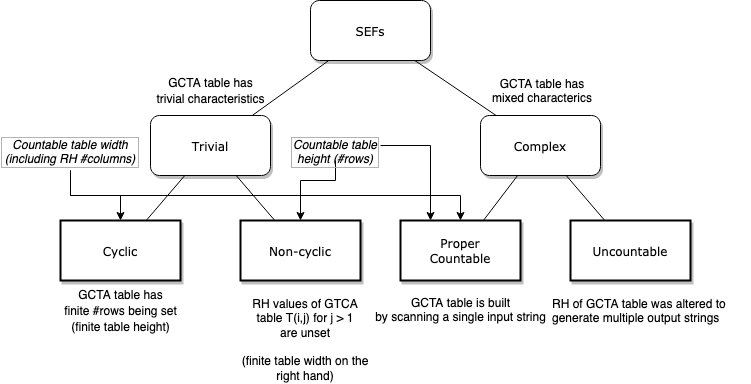
\includegraphics[width=\linewidth]{appendix/CategoriesOfSEFs.png}
  \end{subfigure}
  \caption{Categories of SEFs}
  \label{fig:sefcat}
\end{figure}

Following SEF notation one can define an infinite binary string by combining multiple formulas. A new category, presented in the above figure, is called \textit{complex} and has not yet been discussed. Indeed, according to the proposed categorization a mixture of two trivial SEFs, the cyclic or non-cyclic strings, will produce a GCTA table inherently combining their characteristics. Let us provide an example for it.

\begin{table}[ht]
  \caption{Example of a proper countable GCTA table for complex $\bos(01)(0)\eos$}
  \centering
  \begin{tabular}{ |c|r|l| }
    \hline
    \# & LH                 & RH              \\
    \hline
    1  & $\bos(01)\eos$     & $\bos(0)\eos$   \\
    2  & $\bos(01)0\eos$    & $\bos1(0)1\eos$ \\
    3  & $\bos(01)00\eos$   & $\bos0\eos$     \\
    4  & $\bos(01)000\eos$  & $\bos0\eos$     \\
    5  & $\bos(01)0000\eos$ & $\bos0\eos$     \\
    .. & ..                 & ..              \\
    \hline
  \end{tabular}
  \label{Tab:ComplexGCTA}
\end{table}

Let $b=\bos(01)(0)\eos$ be a bi-infinite binary input string. After scanning it with GCTA one obtains a proper countable table (as illustrated in table \ref{Tab:ComplexGCTA}). The mixed properties here are that the width and height of the table placeholders is both countable and set. In particular, first lines (\textit{\#1 and \#2}) contain cyclic formulas which expand infinitely to the right\footnote{validate RH value $1(0)1$ at line \textit{\#2} for yourself}. Now next lines do not have values of the RH placeholders set starting with the column index $j > 0, j \in J, J \subset \integers$. Although $b=\bos(01)(0)\eos$ consists of two trivial cyclic strings, it is not trivial by itself. In the sense of proposed categorization, GCTA table characteristics observed are similar to both cyclic string $\bos(01)\eos$ in the first lines and non-cyclic string $\bos[1+]\eos$ for the rest.

\subsection{Context argument}

We start by scanning a bi-infinite non-trivial binary string $b = \bos(0)[1+]\eos $ and producing a proper GCTA table $T(i,j)$.

The left-hand of $T(i,j),  \forall j < 0$ will contain all left-infinite strings  observed during scanning of $b$ by construction. Based on the characteristics of non-trivial infinite binary strings the right-hand of $T(i,j),i \in I, I \subset \nat, j \in J, J \subset \integers$ will exhibit both trivial non-cyclic and cyclic characteristics. This means we will have at least one cyclic-like bi-infinite entry $\bos(0)1\eos$ obtained by scanning $\bos(0)\eos$ resulting from zero-padding of $b$ on the left (see line \#1 in table \ref{Tab:GCGA})).

The other part of $b = \bos..[1+]\eos $ generates a unique countable sequence, which is continuously appended on the right. Scanning bits of this infinite sequence results in a list of countably many prefixes on the left-hand of $T(i,j),  \forall j < 0$. The corresponding right-hand entries will be unset for all $\forall j > 0, i > 1$  in $T(i,j)$.


\begin{table}[ht]
  \caption{Initial configuration with proper GCTA table for complex $\bos(0)[1+]\eos$}
  \centering
  \begin{tabular}{ |c|r|l| }
    \hline
    \# & LH                      & RH             \\
    \hline
    1  & $\bos(0)\eos$           & $\bos(0)1\eos$ \\
    2  & $\bos(0)1\eos$          & $\bos0\eos$    \\
    3  & $\bos(0)10\eos$         & $\bos1\eos$    \\
    4  & $\bos(0)101\eos$        & $\bos1\eos$    \\
    5  & $\bos(0)1011\eos$       & $\bos0\eos$    \\
    6  & $\bos(0)10110\eos$      & $\bos1\eos$    \\
    7  & $\bos(0)101101\eos$     & $\bos1\eos$    \\
    8  & $\bos(0)1011011\eos$    & $\bos1\eos$    \\
    9  & $\bos(0)10110111\eos$   & $\bos0\eos$    \\
    10 & $\bos(0)101101110\eos$  & $\bos0\eos$    \\
    11 & $\bos(0)1011011100\eos$ & $\bos1\eos$    \\
    .. & ..                      & ..             \\
    \hline
  \end{tabular}
  \label{Tab:GCGA}
\end{table}

Note that at this point string lists on both left-hand $LH = {T(i,j): j < 0}$ and right-hand $RH = {T(i,j): j >= 0}$ share the same cardinality due to line-by-line\footnote{one-to-one and onto} correspondence. We will denote them as $|LH|$ and $|RH|$ respectively. Both are countable $|LH| = |RH| = |\nat|$.

We will refer to the above setup as an \textit{initial configuration} and use it as a starting point for some proofs below\footnote{many similar configurations are equally acceptable for our purposes}. Will also refer to Cantor's slash argument\footnote{for example, as offered in comprehensive introductory overviews into the concept such as \cite{penrose2007road}} as well as employ some well accepted notations from the theory of smaller and Large Cardinals\footnote{namely, $\aleph_0=|\nat|$ - also see next section for more detailed recap of existing results and notations}.

For convenience, we will refer to the output result of GCGA as a table $T^\prime(i^\prime,j^\prime) = GCGA(b, T(i,j))$ containing those accessible strings or equivalently as to the left-hand $LH^\prime = T^\prime(i^\prime,j^\prime), j^\prime < 0$ and the right hand $RH^\prime = T^\prime(i^\prime,j^\prime), j^\prime \geq 0$. Like that we will treat $T^\prime(i^\prime,j^\prime)$ as a cursor function and sometimes abuse or omit the index notation by meaning enumeration in a wider sense as $\forall i^\prime \in I^\prime, I^\prime \supseteq \nat$ and $\forall j^\prime \in J^\prime, J^\prime \supseteq \nat$ when discussing $T^\prime(i^\prime,j^\prime)$.

Now let us describe how GCGA can act on the initial configuration by assigning values to the previously unset placeholders on the right-hand $RH = {T(i,j): j >= 0}$ in order to produce unobserved state and generate the multitude of output strings (\textit{GCGA steps}):

\begin{enumerate}
  \item create a reference of $T(i,j)$ from the initial configuration as $T^\prime(i^\prime,j^\prime)$ which is both relative to original $T(i,j)$\footnote{acts as copy of $T(i,j)$} and otherwise contains the same values except that it can also be modified or expanded with new placeholders at need so that all indexes are respectively relabeled;
  \item start moving the cursor in the top-down direction from the point closer the top-middle of the $T^\prime(i^\prime,j^\prime)$ by examining values at $i^\prime = 0, j^\prime = 1$ on the right hand of the proper table;
  \item continue to increment access index $i^\prime$ until one can find the placeholder for the state value that has not yet been set at some $i^\prime \geq 0, j^\prime \geq 1$\footnote{optionally and in case of other input strings, one can also increment j up to some finite size of the SEF formula in the state (if desired) and look further on the right for the unset placeholders};
  \item if the values for $j^\prime > 0$ are unset, this means that the prefix on the same counter-part line on the left has been observed only once. Then one can label this location as \textit{suitable for modification};
  \item next, GCGA can be run similar to GCTA steps to output the result with some difference in conditional logic as explained below;
  \item continue with generation on every line by switching between context prefixes
  \item if the the line at index $i^\prime$ can be marked as \textit{suitable for modification}, then:
        \begin{enumerate}
          \item mark corresponding prefix in the LH of $T^\prime(i^\prime,j^\prime), j^\prime<0$ as copied, so that only the finite reference is stored\footnote{we interpret output with such finite separator reference as "multi-lined"}
          \item keep expanding $T^\prime(i^\prime,j^\prime)$ with copies of the marked string including the unset placeholder on the right, preparing them for the modification at the next steps
          \item continue to run the necessary number of iterations for that $i^\prime$ so that one can cover the entire space of yet unset placeholders on the right-hand of $T^\prime(i^\prime,j^\prime), j^\prime>0$ by some countable index mapping $k \rightarrow (i^\prime,j^\prime), k \in K, K \subset \nat$
          \item once you run as many finite iterations of SEFs enumeration for each index pair $(i, j)$  as required by the above one-to-one and onto mapping, append newly obtained binary values to the unset placeholders on the right of $T^\prime(i^\prime,j^\prime), j^\prime > 0$
          \item optionally, generate an output string each time the new placeholder is appended
          \item update $(i^\prime,j^\prime)$ for the next iteration of the cover on the same line either by remembering values or computing them from the cover mapping
          \item continue to loop over the covering map $k \rightarrow (i^\prime,j^\prime)$ to repeat the above sub-process from step 3 as many times as necessary\footnote{up to countably many times} or until you have reached the output values desired by the access or a cursor function
        \end{enumerate}
\end{enumerate}

Keep in mind, that every appending (generation) happening in the steps 7(c) and 7(d) of \textit{GCGA steps} over previously unset values is interpreted as access (generation) of a new output infinite binary string which continues to expand with the new unobserved part of the prefix \footnote{due to construction of the algorithm}. Unless designed, the described algorithm will never terminate for the specific input string $b = \bos(0)[1+]\eos$. In fact, this is not necessary for our purposes as it is enough to show that:
\begin{itemize}
  \item the above description of GCGA algorithm generates new unique strings from the point of view of the particular "fork" or branch starting at some $(i^\prime,j^\prime)$
  \item as well as provides the ability to access the necessary values at the exact "fork" or branch observed after the given context in $LH$
\end{itemize}

It is easy to see that GCGA can be further modified to print out only desired or finite parts of the output. Recall, that we refer to such output strings as algorithmically reachable by a cursor.

We can observe that after applying GCGA to the $T(i,j)$, the table will not be proper anymore in a sense that the left-hand $LH^\prime$ contains duplicates, which are still unique strings only if considered jointly with their right-hand counter-parts in $RH^\prime$ list.

It is important to stress the following fact again - the property that makes every new string listed in the table $T^\prime(i^\prime,j^\prime)$ unique is the peculiar design of GCGA, which goes beyond counting\footnote{in a sense of recursive construction of natural numbers $\nat = \{x_{i+1} = x_{i} + 1\}, \forall i \in I$} and is simply a special way of accessing every traversable object that can be output by the algorithm with or without given context in $LH$.


We have reached the point when we know how $T^\prime(i^\prime,j^\prime)$ can work by applying GCGA to $T(i,j)$ values. It is still not clear if left and right "table halves" when accessed via the respective cursor functions $T(i,j)$ and $T^\prime(i^\prime,j^\prime)$ can result in producing the output of the same left and right cardinality $|LH| \stackrel{?}{=} |RH^\prime|$ or alternatively can access parts of one or more unique bi-infinite binary strings which we can show to be unequal.


\begin{theorem}
  Let $T^\prime(i^\prime,j^\prime) = GCGA(b, T(i,j))$, where both $T^\prime(i^\prime,j^\prime)$ and $T(i,j)$ are cursor functions as well as $T(i,j)$ is a proper table over input bi-infinite binary string $b$ and $b$ is proper countable. Cardinality of $|LH| < |RH^\prime|$ when accessed via $T(i,j)$ and $T^\prime(i^\prime,j^\prime)$ from input $b$ respectively.
\end{theorem}

\begin{proof}The above statement  $|LH| < |RH^\prime|$ can have a meaningful answer only when we recall that $T^\prime(i^\prime,j^\prime)$ tries not just to access but also to generate new elements in the sense of the algorithm application explained above in \textit{GCGA steps}. Let $b = \bos(0)[1+]\eos$ or any other proper countable input string. Proceed with initial configuration and apply GCGA steps to $T(i,j)$ proper table constructed with GCTA. We can produce any arbitrary or specifically requested output range through means of the cursor $T^\prime(i^\prime,j^\prime)$.

  Now let us show that the resulting output of applying GCGA will fall into the category of the proper uncountable strings. We can point out the exact difference in the end result of the traversing process up to specific index. In order to do so, choose any nearest $(i^\prime,j^\prime)$ index pair suitable for modification (\textit{GCGA step 7.c}). Observe that $j^\prime > 0$ meaning the cursor is pointing at the yet unset placeholder in both $T(i^\prime,j^\prime)$ and $T^\prime(i^\prime,j^\prime)$. Select the row $i^\prime$ from $T(i,j)$ table without any unset values as a left-infinite string $a := (T(i^\prime,j), \forall j < j^\prime)$. Iterate further through GCGA steps to pick next suitable value $v \in \{0, 1\}$ from the generation scheme (or pattern, such as "[1+]"). Assign that value at the cursor $T^\prime(i^\prime,j^\prime) := v$. Select the row from $T^\prime(i^\prime,j^\prime), \forall j^\prime$ without any unset values as a left-infinite string $a^\prime$. Observe that $a^\prime \neq a$ and is different up to a single placeholder that is still unset in $T(i^\prime,j^\prime)$. Then notice that string $a$ is also a prefix of $a^\prime$ as in $a = ".., a^\prime[j^\prime-2], a^\prime[j^\prime-1]"$. If $a^\prime \notin T$ table, then $|LH| < |RH^\prime|$. Indeed, assume the opposite that $a^\prime \in T$. By design of GCTA the $T(i,j)$ table is constructed as proper, meaning that $T(i^\prime,j^\prime)$ can have multiple states assigned for the prefix of $a$ in $RH$ iff the prefix of the left-infinite string $a$ is observed in $b$ multiple times. The latter is not the case. Neither prefix of $a$ nor $a$ is observed in $b$ more than once, hence $a^\prime \notin T$.

  This new string $a^\prime$ has been just appended to $T^\prime$ table by GCGA, so that $i^\prime := i + 1$. We can continue to generate similar new and unique strings and access them by means of the $T^\prime(i^\prime,j^\prime)$ cursor an exact and finite number of times\footnote{by design and implementation of GCGA}, until we switch to the next index suitable for modification. However, that means that $RH^\prime$ is strictly uncountable and $|LH| < |RH^\prime|$. \end{proof}

One should avoid confusions in interpreting the results stated in the \textit{Theorem 10}. We have shown that one can use GCGA \footnote{or similar schemes} to achieve algorithmic accessibility when it comes to handling larger objects arranged from infinite binary strings. Such schemes can be used to construct and access objects like $RH^\prime$ demonstrating to have the property of strictly greater cardinality over $|\nat|$. However, if we run GCGA implementation on a deterministic TM any produced output will be naturally of the same countable cardinality, just as the one of GCTA \footnote{with the only difference in the printed-out values}. We are again in need of tools that can help us operate with such objects of greater uncountable cardinality more intuitively.

\subsection{Uncountable cardinalities}

In the previous section (see - \textit{Theorem 10}) we have indicated yet another way\footnote{next to natural numbers as well as transfinite cardinal and ordinal numerals - read further for more detailed explanation} for how to count at infinity or expand upon large objects such as lists of infinite binary strings. Next, we will reference and introduce some more of notation to be able to discuss previously known theory and its results. Our intention is to better understand potential consequences of such presumably novel "counting" technique.

We begin by following into the original line of thinking as offered by George Cantor. Cantor introduces a theory for transfinite numerals called ordinals and defines their cardinalities. He also famously introduces the Cantor's diagonal or slashing argument\footnote{Further we will refer to Cantor's diagonal argument simply as \textit{slashing}}. The idea behind slashing is to compare cardinalities of rather large objects such as infinite lists of items by employing the bijective mapping\footnote{An instructive overview of these and other ideas by Cantor\cite{cantor1915contributions} for matching cardinalities (starting with $|\rationals| = |\nat|$) has been cleverly outlined in "Hilbert's Hotel" by Gamow\cite{gamow1988one}, p.17.}. 

Bijective mapping of objects is such a central tool to the discussion of cardinality (in the proposed set theory by Cantor and beyond) that we want to state it even more formally as a principle.
\begin{principle}[Principle of one-to-one correspondence]\label{principle_1to1_cor}
  Objects have the same cardinality if and only if their elements are in one-to-one correspondence. 
\end{principle}
One-to-one correspondence between objects is usually proved by showing the existence of the respective bijective mappings or, equivalently, functions which are both one-to-one and onto\footnote{Also see the set theoretical definitions for bijective functions as discussed, for example, in\cite{goldrei1996classic, kunen1980set, jech2003set}}.

Again, this principle turned out to be very insightful and helped to make sense out of many less-intuitive situations when objects were looked upon much more restrictively - for example, only from the perspective of trivial counting. Let us recap on that.

Recall that counting procedure provides us with the set of natural numbers $\nat = \{1, 2, 3..\}$. Any taken subset of natural numbers $ X \subset \nat$ will be always limited by some largest number at the very end of such subsequence $X$, meaning that the cardinality of such subset is finite $|X| < |\nat|$. However since the sequence of the natural numbers $\nat$ by itself is always constantly appended with a new number which will be an increment of the previously seen largest number, we say that the cardinality of natural numbers is actually infinite and corresponds to the countable form of infinity. This can be captured by assuming the existence of some transfinite limit $\omega_{0}$\footnote{$\infty$ sign was suggested to be replaced by Cantor with $\omega$ which is a less confusing notation\cite{cantor1915contributions}}. This limit $\omega_{0}$ is strictly greater than any natural number\footnote{which is also a definition of any transfinite numeral - see \cite{jech2003set} for much better introduction into ordinals} and will be a first transfinite number such that if $X^\prime \subseteq \nat \cup \{\omega_{0}\} $, then we say such subset has a first infinite or countable cardinality similar to that of natural numbers. Cardinality of sets that include ordinal limits is notated with aleph letters. For example, for the inclusion of the first ordinal limit $\omega_{0}$ we use $\aleph_{0}$ and say $ \aleph_{0} = |X^\prime| = |\nat|$. The idea of transfinite numbers gets further developed by introducing the theory of \textit{ordinal numbers}\cite{cantor1915contributions}.

A set of natural numbers consist of elements which can be counted and hence \textit{well-ordered}. Counting provides order-preserving bijection for well-ordered sets by labeling\footnote{and simply agreeing that the order of some elements is greater than the others}. Each cardinal number can be related to some limit ordinal of the underlying set. For example, for natural numbers\footnote{by re-ordering a set we can assign it a new order type} that would be a first order type $\omega_{0}$\footnote{mind the index at omega for convenient mapping with alephs further on}. Thus we say that any of the ordinals starting with $\omega_{0}$ in the well-ordered sequence $\omega_{0},\ \omega_{0} + 1,\ \omega_{0} + 2,\ ..  $ will be strictly greater than any natural number. All $\omega_{0}$ ordinals such as $\{\omega_{0},\ \omega_{0} + 1,\ \omega_{0} + 2,\ ..\}$ correspond to the first transfinite cardinal $\aleph_{0}$. Similar association is true for the next biggest transfinite cardinal $\aleph_{1}$, to which all $\omega_{1}$ ordinals such as $\{\omega_{1},\ \omega_{1} + 1,\ \omega_{1} + 2,\ ..\}$ can be mapped to as many to one\footnote{in most frameworks like Zermelo–Fraenkel (ZF) set theory this usually requires an \textit{Axiom of replacement}}. We say that $\aleph_{1}$ is a first transfinite cardinal for the infinite set with uncountable cardinality.

Although $\omega_{0}$ and $\omega_{0} + 1$ have different respective order types, they do not add more to the original cardinality $\aleph_{0}$ of the corresponding set $\nat$\footnote{keep in mind that re-ordering the set does not change its cardinality, even in case of transfinite sets}. To reiterate over the idea of cardinalities of ordinal transfinite numerals again - indeed, if ordered set $\nat \cup \{\omega_{0}\} = \{0, 1, 2, 3, .., \omega_{0}\}$, then the cardinality $|\nat \cup \{\omega_{0}\}|$ is still the same as $|\nat| = \aleph_{0}$.

Recall that ordinals are defined as order preserving sets, but transitive addition in ordinal arithmetic is not commutative\footnote{contrary to the definitions of ordinal arithmetic and in case if natural ordinal arithmetic is applied, one can achieve $1 + \omega_{0} = \omega_{0} + 1$ }. One can still have the well-ordering in form of right-side addition as in $\omega_{0} < \omega_{0} + 1$, even though it is not the same for left-side addition when $1 + \omega_{0} = \omega_{0}$. This means that applying ordinal arithmetic will not result in order preserving bijections between $\nat \cup \{\omega_{0}\}$ and $\{\omega_{0}\} \cup \nat$. Namely, the later will have order type $1 + \omega_{0} = \omega_{0}$, based on the bijection $\{\omega_{0} \rightarrow 0, i \rightarrow i + 1 : \forall i \in \nat \}$, and hence $1 + \omega_{0} < \omega_{0} + 1$.

Other interesting insights that we want to recap are based on the concept of powerset. This concept is a helpful example of yet another way to count things at infinity (next to transfinite ordinals). The concept itself is as following, if $X$ is a set of items, then a set $\pset(X)$ consists of all subsets of set $X$ and is called a \textit{powerset} of $X$.

Numbers can be constructed from sets. For example, applying only empty set one can show how to construct natural numbers \cite{penrose2007road}. The process of recursive application of \textit{powerset} to sets with cardinalities of $\aleph_0$ and larger is called \textit{transfinite exponentiation}. It can be also used to construct \textit{ordinals} from sets\footnote{for other than Cantor ordinals, please check von Neumann ordinals with an alternative proper-class construct: "each ordinal is the well-ordered set of all smaller ordinals"}. Such sets are referred to as \textit{omega sets}\footnote{mind the $\omega$ letter we have used earlier} of well-ordered numerals and can be used to show how greater orders of infinity (beyond countable) can be set up\footnote{ultimately by stating the existence of transfinite numerals as we have done earlier, see - \textit{"The Transfinite Ordinals and Cantor’s Mature Theory. In: Labyrinth of Thought"}\cite{ferreiros2008labyrinth}, pp. 257-296 as well as \cite{kanamori1996mathematical}}.

However, one has to be careful when working with such concepts as \textit{set of sets}. It has been proven to be unexpectedly complex and may easily lead to paradoxes\footnote{For example - \textit{Russell's paradox}} if no special considerations are put in place\footnote{For instance - the requirement to operate within certain logical framework which relies on axiomatic systems such as ZF set theory}. Whenever possible we will replace the notion of \textit{set of sets} either by considering \textit{lists of items}, where items are more concrete objects than sets such as binary strings or by simply looking at classes of numerals\footnote{Meaning that we try to implicitly employ the proper-class construct as proposed by ZF everywhere in our discussion}.

The powerset concept is used in another important result called Cantor's Theorem \footnote{see \cite{jech2003set} and for conceptual proof outline refer to \cite{penrose2007road}}:

\begin{theorem}If $|X| = \alpha$, then $|\pset(X)| = 2^\alpha$ and $\alpha < 2^\alpha$, where $2^\alpha$ is the total number of subsets of any set such as $X$.\end{theorem}

As a consequence one can state\footnote{Alternatively, one will rely on the proof using Cantor's diagonal argument\cite{penrose2007road} applied to the list of all binary strings} the existence of strictly greater cardinality $\aleph_{0} < 2^{\aleph_{0}}$. An assumption that $\aleph_{1} \stackrel{?}{=} 2^{\aleph_{0}}$ is equivalent to the \textit{continuum hypothesis}\footnote{Assuming the axiom of choice, there is the smallest cardinal number $\aleph_{1}$ greater than $\aleph_{0}$, and the \textit{continuum hypothesis} is in turn equivalent to the equality $\aleph_{1} = 2^{\aleph_{0}}$\cite{goldrei1996classic}.}, which needs more explanation.

We define the cardinality of real numbers as $\cont = |\reals|$. Cantor gave two proofs that the cardinality of the set of integers is strictly smaller than that of the set of real numbers $\aleph_{0} < \cont$\footnote{Cantor's first uncountability proof and Cantor's slashing}. However, those proofs provided no indication to which extent or how far does the difference of cardinality in $\aleph_{0} < \cont$ goes, so Cantor has proposed the continuum hypothesis (CH)\footnote{see \cite{jech2003set, herrlich2006ac} as well as \cite{enwiki:1062726958} for more informal but comprehensive covering} as a possible solution to this question. The CH states that there exists no set $S$ for which $ \aleph_{0} < |S| < \cont$\footnote{which is a weaker version of the CH formulation}.

\subsection{Formal SEF languages}

So far we have provided a number of definitions to describe infinite binary strings. Good news is that our discussion and results are not based on dealing with highly abstract sets\footnote{and equally large, such as \textit{von Neumann universe} in ZFC} yet, but rather with concrete objects like lists of binary strings\footnote{residing and computable within the realm of theoretical computer science}. This means we did not rely much on any foundational framework\footnote{such as ZFC}, so the results in \textit{Theorem 10} are mostly independent. Unfortunately at this point such results are still not formal enough to explain what exactly do we mean by \textit{uncountability} or how to interpret our claims about cardinality of inspected objects. Instead of moving forward with developing a complete theory of infinite binary strings from scratch\footnote{in terms of mathematical logic} by doing further build-up on presented GCGA concept, we intend to harden and refine our definitions referencing something well-known. We will do so by obtaining an exact explanation based on already existing results in classic set theory\footnote{which we have most briefly recapped and referenced in the previous section - also see \cite{goldrei1996classic}} and theoretical computer science\cite{Sipser05introcompther}.

With such motivation in mind, this subsection will focus on refining definitions of SEFs as formal languages\footnote{following Chomsky hierarchy}. Next subsection will describe an algorithm that we will refer to as \textit{continuum access scheme} (CAS) and benefit from the definitions.

Recall that in computer science\cite{Sipser05introcompther} a formal language is defined over some alphabet. An alphabet is usually a finite set or list of symbols or sometimes strings. For example in both cases, $\Sigma=\{0,1\}$ or $\Sigma=\{ab,ba,c\}$ are alphabets.

\begin{definition}
  If $\Sigma$ is a finite set of strings called alphabet, then $\Sigma^*$ is an infinite list of all possible concatenations over those strings, s.t. $|\Sigma^*| = \aleph_0$.
\end{definition}

The star symbol notation used in $\Sigma^*$ is called Kleene-closure of $\Sigma$. Alternatively, $\Sigma^*$ is said to be closed under string concatenations including the empty string $\epsilon$\footnote{a zero length string, similar to the empty set element}.

A formal language consists of \textit{words} whose letters are taken from an alphabet and are \textit{well-formed} according to some specific set of rules.

\begin{definition}
  If $\Sigma$ is a finite alphabet, then a \textit{formal language} $L$ over an alphabet $\Sigma$ is defined as a set $L := \{ w\ is\ valid : \forall w \in \Sigma^* \}$, where each word $w$ is a \textit{well-formed} or \textit{valid} expression of $L$.
\end{definition}

Words of formal languages can be also referred to as expressions or formulas. Now we want to take a closer look at what does the {well-formed expression} means or the notion of formula validity for SEFs by summarizing what has been discussed about SEFs so far as a set of rules.

\begin{definition}
  A formula $\phi$ is a valid String Enumeration Formula iff all of the following is true:

  \begin{enumerate}
    \item $\phi$ is an input-free program generating an infinite binary string as an output in countable time\footnote{meaning that number of output characters or the cardinality of the output is never greater than $\aleph_0$ - also see \textit{Definition 11}}
    \item formula has always a finite length $|\phi| = m: m \in \nat$ unless specified otherwise\footnote{one can explicitly specify countable length for $\phi, |\phi| = \omega_0: \omega_0 > n, \forall n \in \nat$}
    \item replicator syntax is a balanced pair of round brackets such that number of balanced bracket pairs is finite $|\phi|_{(} = |\phi|_{)} = n: n \geq 0, n \in \nat \cup \{0\}$
    \item round brackets can be nested which is interpreted as recursive replicator calls
    \item a replicator can not be defined over an empty string
  \end{enumerate}
\end{definition}

Given the notion of SEF validity we can define a \textit{didactic} procedure as an algorithm accepting only valid input expressions. This also allows stating the definition of a formal language for SEFs.

\begin{definition}A Formal String Enumeration Formula language or \textit{SEF language} is a formal language constructed from syntactically valid formulas over alphabet $\Sigma$ as $L_{SEF} := \Delta(\Sigma^*)$, where $\Delta$\footnote{do not confuse with $\Delta_0$ formulas\cite{jech2003set} of first order logic} is a validation procedure or \textit{didactic} that can recognize only well-formed expressions of $L_{SEF}$. $\Sigma := V \cup \gamma$ is a union between set $V$ of vocabulary symbols and set $\gamma$ of syntactical symbols (syntax).\end{definition}

One can state an equivalent definition.

\begin{definition}$L_{SEF}$ is a \textit{SEF language} constructable from a tuple $(\Sigma, \Delta)$ iff $\Delta \subset \Sigma^*$ s.t. all formulas in $\Delta$ must be both syntactically valid and computable as SEFs.\end{definition}

Note that for most purposes formal languages are defined over finite alphabet. The same is with SEF languages unless specifically considered.

\begin{definition}If $L_{SEF} := (\Sigma, \Delta)$ is a SEF language and $\exists k \in \nat: |\Sigma| \leq k$, then we say that $L_{SEF}$ has an alphabet with finite cardinality $k$.\end{definition}

This is different from the cardinality of the language which is a set of all valid formulas.

\begin{definition}If $L_{SEF} := (\Sigma, \Delta)$ is a SEF language then the cardinality of the language is the same as $|\Delta|$.\end{definition}

Finally, we say that the language is finite if it can recognize strings of finite length.

\begin{definition}If $L_{SEF} := (\Sigma, \Delta)$ is a SEF language and each formula of the language is finite $\forall \phi \in \Delta: |\phi| \leq n, n \in \nat$ then we say that $L_{SEF}$ is a finite language.\end{definition}

\begin{theorem}
  If $L_{SEF} := (\Sigma, \Delta)$ is a finite SEF language then $L_{SEF}$ is also a regular language.
\end{theorem}
\begin{proof}
  Recall the result from \cite{Sipser05introcompther} that every formal language is a regular language iff it can be recognized using a regular expression. Observe that regular expressions themselves form a regular language or can be parsed by a regular expression. Since every SEF expression can be reduced to a regular expression by mapping replicator syntax to a Kleene-closure, it means that there exists a regular expression to parse SEFs.
\end{proof}

Obviously, even if both the cardinality of the alphabet\footnote{i.e. $| V \cup \gamma| \geq \aleph_{0}$} and the cardinality of the SEF language itself\footnote{language contains formulas of countable length} is infinite, it can be still restricted by some greater cardinality unless shown or defined otherwise.

Please note that so far we have been working only with finite SEF languages and will continue to do so. For example, $L_{SEF} := (\Sigma, \Delta) = (\{0,1\} \cup \{{(}, {)}, {:}\}, \Delta)$ is a finite SEF language equipped with round brackets as replicator symbols and colon for access symbol and $\forall \phi \in \Delta: |\phi| \leq n, n \in \nat$. If needs be, the extended version of the syntaxes may include square brackets for binary conversion of in-line decimals as well as plus and star generating short-hands for enumeration scanning.

Next we would need one more definition to count how many times one sub-string can occur in another string.

\begin{definition}Given $L_{SEF}$ is a SEF language and $\exists z,s: z,s \in \Delta$ are valid strings in that language, such that one string can occur in another one at least once, i.e. $z \in s$. This fact is noted as $|s|_{z}$ and is called cardinality of $z$ in $s$.\end{definition}

In case when we can count how many times one sub-string can occur in another string, then this is noted as $|s|_{z} = \lambda: \lambda \in \nat$.

\subsection{Continuum access scheme}\label{subsec_cas}

We base on the setting similar to the GCGA initial configuration. We start by scanning a string $b=\bos(0)[1+]\eos$ with a small difference in approach but without loss of generality. Instead of scanning bit by bit, we jump over the full binary representation from one integer $\bos(0)[1][2]\eos$ to the next one $\bos(0)[1][2][3]\eos$. Such scanning is marked as $b=\bos(0)[1*]\eos$. Like that all bits of each integer are concatenated at full for every string we add to $LH$ of the table (see fig. \ref{fig:continuuma}).

\begin{figure}[h!]
  \centering
  \begin{subfigure}[b]{0.9\linewidth}
    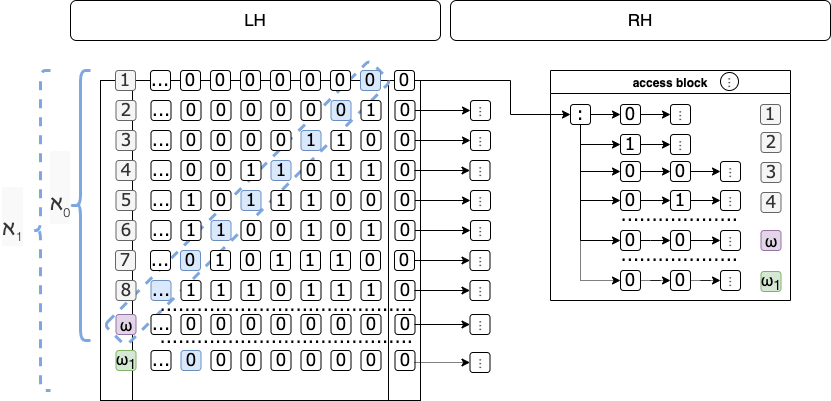
\includegraphics[width=\linewidth]{appendix/access-scheme.png}
  \end{subfigure}
  \caption{Continuum access scheme}
  \label{fig:continuuma}
\end{figure}

We also extend the SEF formula language of infinite binary string enumeration using a colon symbol. On the $RH$ of the table we have something called \textit{access block} labeled with three vertical dots. The expanded version of this block contains the access step noted with colon symbol. Keep in mind that the access block is recursive. For example, a string formula that indicates some instance of algorithmic access from the $LH$ context with the span into the $RH$ is designated as $\bos(0)[1]{:}01{:}010({:}0)\eos$, where the string replicator on the very right end $\bos..({:}0)\eos$ represents a continuous access action into the $RH$. When one needs to compute such an infinite binary string formula, one can imagine a computation process by expanding each replicator without stop. The replicator with the access colon symbol means continuous recursive access with ever expanding context on the left hand of each colon. This schematic representation describes nothing else but the recursive application of the GCGA and can be seen as yet another generalization step through the employment of the recursive definition.

On one hand, we don't necessarily need to restrict number of times when the colon symbol appears in such extended SEF notation. Indeed, such cases can be called an infinite algorithmic access scheme or simply \textit{continuum access scheme}. On the other hand, if we would prefer to restrict number of occurrences for the colon symbol by some finite limit, that should be possible as well.

Now let us consider another simplification with the finer subcase of applying continuum access scheme (see fig. \ref{fig:continuuma}) but only a limited number of times.

\begin{definition}If $L_{SEF} := (V \cup \gamma, \Delta_\delta)$ is a finite SEF language, which syntax is equipped with a colon as an access symbol and any formula in its didactic set $\Delta_\delta$ contains colon symbol but only limited number of times, then we say that language $L_{SEF}$ has some finite depth of $\delta$. Specifically, $\exists \delta \in \nat, \forall s \in \Delta : |s|_{{:}} \leq \delta$.\end{definition}

Access schema for languages with finite depth can be imagined as similar to fig.\ref{fig:continuuma} but without having an infinite recursion call inside the access block\footnote{a block with the three vertical dots symbol}. Number of calls becomes limited by counting. We are particularly interested in this case as we can show not only that there is no bijection between LH and RH parts of the corresponding computationally expanded GCGA table\footnote{by applying result from \textit{Theorem 10}}, but specifically to extend and pin-point the relationship between LH and RH parts.

Let $L_{SEF} := (V \cup \gamma, \Delta_1)$ be a finite SEF language with a binary vocabulary $V := \{0,1\}$, typical syntax $\gamma := \{{(}, {)}, {:}\}$ and didactic with a single access depth, s.t. $\forall s \in \Delta : |s|_{{:}} = 1$. Consider a proper table with cursor $T(i,j)$ obtained by scanning a proper countable bi-infinite input binary string $b$ and a cursor function $T^\prime(i^\prime,j^\prime)$ such that $T^\prime(i^\prime,j^\prime) = GCGA(b, T(i,j))$ which will allow algorithmic access as exposed in \textit{Theorem 10}. For instance, if $\exists i^\prime,j^\prime: i^\prime \in I^\prime$ and $j^\prime \in J^\prime$ are some indexes and there is a formula $f := \bos(0)1{:}01\eos$ corresponding to $i^\prime \in I^\prime$, then the sub-string before the colon (acting as an access symbol) will correspond to the context of the expanded string accessed via cursor function $T^\prime(i^\prime,j^\prime): \forall j^\prime < 0, j^\prime \in J^\prime$ and will be equal to $\bos(0)1\eos$. While the part after the colon corresponds to the value-state of the expanded string from $T^\prime(i^\prime,j^\prime): \forall j^\prime > 0, j^\prime \in J^\prime$ and will be equal to $\bos01\eos$.

The above approach is similar for finite languages of greater depth. For example, in case of $L_{SEF} := (V \cup \gamma, \Delta_2)$ if there is a formula $f := \bos(0)1{:}01{:}1\eos$, then the whole sub-string before the second occurrence of the colon symbol will correspond to the context when the second access is evaluated. However, for greater clarity we replace multiple-prime notation with depth index. This applies to cursor functions $T_\delta(i,j)$, so that

\begin{align*}
  if\:\delta = 1{:} & \quad T_{1}(i,j) := T^\prime(i^\prime,j^\prime)                            \\
  if\:\delta = 2{:} & \quad T_{2}(i,j) := T^{\prime \prime}(i^{\prime \prime},j^{\prime \prime}) \\
  ... {   }         &
\end{align*}

and so on. Also further we assume that depending on the context the cursor indexes $i, j$ are remapped from their index supersets accordingly. For example, $j^\prime \in J^\prime$  is always re-mapped from $j^{\prime \prime} \in J^{\prime \prime}$\footnote{projected or pulled from the superset - for example, this can be implemented via Levy collapse of cardinals\cite{jech2003set}; we also discuss implementation of CAS in later subsections} via $\alpha: J^{\prime \prime} \to J^\prime$ based on depth and occurrence of the access symbol and given that $J^\prime \subseteq J^{\prime \prime}$. Such mapping is equivalently rewritten as $\alpha: J_2 \to J_1$, where $j_1 \in J_1, j_2 \in J_2, J_1 \subseteq J_2$. The same is true for $LH^\prime$ and $RH^{\prime \prime}$ being rewritten as $LH_1$ and $RH_2$.

\begin{theorem}Let $L_{SEF} := (\{0,1\} \cup \{{(}, {)}, {:}\}, \Delta_\delta)$ be a finite SEF language with a binary vocabulary, typical syntax and didactic with a finite depth $\delta \in \nat$. If a cursor function $T_\delta(i,j)$ implements continuum access schema for $L_{SEF}$ limited by some finite $\delta \in \nat$ for every formula in didactic $\Delta_\delta$, then for every algorithmically accessed value-state sub-string $\forall \nu_\delta \in RH_{\delta+1}: \nu_\delta := T_{\delta+1}(i,j): \forall j > 0, j \in J_{\delta+1}, i \in I_{\delta+1}$ given context $\phi_\delta \in LH_\delta: \phi_\delta := T_\delta(i,j): \forall j < 0, j \in J_\delta, i \in I_\delta$ there exists surjection

  \begin{align*}
    \rho_\delta \colon RH_{\delta+1} & \to LH_\delta       \\
    \nu_\delta                       & \mapsto \phi_\delta
  \end{align*}

  such that at least for $\delta = 0: |LH_\delta| < |RH_{\delta+1}|$ and $|RH_{\delta+1}| \leq |\pset(LH_\delta)|$, where $\pset(X)$ is a powerset of $X$.\end{theorem}

\begin{proof}The theorem is proven by following the construction of the continuum access schema.

  A finite case for the existence of the surjection $\rho \colon RH_1 \to LH$ is trivial. It is enough to show that $\rho: \nu \mapsto \phi$, where $\forall n \in \nat, m \in \{1, .., 2^n\}: \nu = \bos[m]\eos, \phi = \bos[n]\eos$, which is the case for $T_1(i,j)$ table with any finite number of $i \leq 2^n$ lines. Given that the $|\pset(X)| = 2^{|X|}$ if $X$ is a finite set, then the existence of the surjection $\rho \colon RH_1 \to LH$ is satisfied for $LH$ of $T(i,j)$ and $RH_1$ of $T_1(i,j)$.

  For the infinite case we need to consider $|LH| \geq \aleph_0$. This can be achieved by slashing $LH$ as shown on fig.\ref{fig:continuuma}, then adding an inverted diagonal as new string labeled $\omega$ to $LH := LH \cup \{\omega\} $ and extending $RH$ with the link to access block accordingly. So far we have not commented on how the $RH$ part of $T(i,j)$ is expanded. Continuum access is implemented based on Theorem 10 result by recursively applying GCGA as in $T_{\delta+1}(i,j) := GCGA(b, T_\delta(i,j))$, where input $b$ can be ignored after initial application. The role of $RH_{\delta+1}$ extension is performed by the access block, so that each entry in the access block is interpreted as value-state sub-string before the next iteration down the recursive call. Like that value-state of the previous iteration of the access call becomes appended (concatenated) to the new context of the next access call.

  Note that given $L_{SEF}$ and for all countably and recursively extendable cases of $LH_\delta: \delta \in \nat$ the access block always represents an infinite access scheme to all possible infinite binary strings, the cardinality of which by Cantor's theorem equals to $2^{\aleph_0}$ due to existing bijection between the set of all infinite binary strings and continuum of real numbers $\reals$. The same theorem states $2^{\aleph_0} = |\pset(\aleph_0)|$\cite{jech2003set}.

  Both for finite and infinitely recursive access blocks we still rely on the algorithmic access as a possible selective reference to higher value-states of $\delta \geq 1$. Specifically, one can think of $RH_{\delta+1}$ values getting pulled down into $LH_{\delta}$ at need \footnote{only when provided with the specific context}.

  Now in our case, $L_{SEF}$ language is finite and $\delta \leq 1$. Since the access block recursion is called only finite number of times we can only state that the right-hand is not greater than cardinality of the continuum or $|RH_{\delta+1}| \leq |\pset(\aleph_0)|$

  Given that $|LH| = \aleph_0$ and using generalization of Theorem 10 by induction, one has $|LH_{\delta}| < |RH_{\delta+1}|$. This means there exists a surjection  $\rho_\delta \colon RH_{\delta+1} \to LH_\delta$, specifically such that $|LH_\delta| < |RH_{\delta+1}|$ and $|RH_{\delta+1}| \leq |\pset(LH_\delta)|$ at least for $\delta = 0$.\end{proof}

A valid concern would be to ask if such continuum access schema is computable on a general computer or an equivalent TM. The answer is \textit{no} and it follows from the following explanation. Indeed, from computer theoretical perspective this still means that not every infinite binary string can be accessed\footnote{see \textit{halting problem} for details} with existing computers. Another way to say the same is that \textit{every algebraic number is computable} or \textit{every transcendental number is incomputable}\footnote{every Chaitin's constant is the example of incomputable number - also see subsection \textit{Computability of SEF languages}}. Even if one would take a step back to assume the existence of some special-purpose formalism\footnote{uncommon enough, beyond general computer programs} that would permit efficient implementation of the algorithm\footnote{or rather a schema} for the described continuum access schema for all left-infinite countably extendable expansions of contexts in $LH_\delta: \delta \in \nat$ then most likely such algorithm is neither in RE nor in co-RE complexity class\footnote{this however should be more carefully reviewed for the $\omega$-regular languages and respective "$\omega$-RE" class if only such can be meaningfully defined for some extended version of Chomsky hierarchy}.

One can notice that once we have applied slashing to $LH$ (see fig.\ref{fig:continuuma}) as according to the explanation in the above proof, we can repeat the process to obtain $\omega_1$ string and produce an uncountable extension of $|LH| = \aleph_1$. Technically there is nothing stopping us from doing so at this point. Another peculiarity is that the proof of Theorem 12 was obtained only for the case of at least $\delta = 0$, without full generalization by induction. The reason behind this is a valid concern that we don't necessarily know yet how big is exactly the cardinality of the continuum $\cont = 2^{\aleph_0}$. In fact, besides highlighting such concern, the Theorem 12 does not provide any additional insights except already known results due to Cantor's work\cite{cantor1915contributions, kanamori1996mathematical, goldrei1996classic}. However, we did manage to provide an illustration of relation between cardinalities of $\aleph_0$, $\aleph_1$ and $2^{\aleph_0}$ in form of continuum access schema using infinite binary strings as well as the connection to the set theoretical axioms\footnote{ultimately, by building up on the result of Theorem 10 - so that uncountability concept is fully aligned with the original set theoretical notion by Cantor}.

\subsection{Uncountability of SEF languages}

On one hand we have looked at the definitions of formal SEF languages which have a finite alphabet and consist of countably many formulas of finite length. This aligns nicely with the well-known formalism in computer science theory such as regular languages. On the other hand, the motivation behind SEFs was to have an expression which produces an infinite binary string. But if we want to expand on our understanding of uncountability, we would need to look into extending the definition of formal SEF languages to be able to handle expressions of infinite length.

Let us revise some properties of the formulas in a finite SEF language $L_{SEF} := (\Sigma, \Delta)$. Each valid $\phi \in \Delta$ can be computed into some infinite binary string $b \in \cbin, |b| = \aleph_0$ to produce an output. In fact, the opposite is also possible if one needs to take some infinite binary string $b \in \cbin, |b| = \aleph_0$ as an input and recognize it by an $\omega$-regular expression\cite{Staiger1997}.

\begin{lemma}
  If $L_{SEF} := (\Sigma, \Delta)$ is a finite SEF language of countably infinite cardinality $|L_{SEF}| = |\Delta| = \aleph_0$, then each finite and valid $\phi \in \Delta, |\phi| = k, \forall k \in \nat$ is itself an $\omega$-regular language that contains exactly one binary infinite string it can recognize.
\end{lemma}

\begin{proof}
  By definition in \cite{Sipser05introcompther}, $\Gamma^*$ is a formal language iff it is an infinite list or a sublist of all possible finite strings built over some alphabet $\Gamma$. If one considers infinite words or $\omega$-words they will constitute an $\omega$-language. Similar to regular languages, $\omega$-language is $\omega$-regular iff it can be recognized using an $\omega$-regular expression. This can be shown by replacing replicator in each $\phi \in \Delta$ with the $\omega$-Kleene closure as defined for the $\omega$-regular expressions. Since $\phi$ can produce only one infinite (countable) binary string when computed as SEF, the corresponding $\omega$-regular language will also contain only one such string.
\end{proof}

However, the above still means that a single infinite binary string can be recognized by a multitude of $\omega$-regular expressions or many $\phi \in \Delta$ formulas. But each SEF $\phi$ produces only one infinite binary string. Again, given that $\cbin$ is a list of all infinite binary strings, then such mapping as $f : \Delta \to \cbin$ is not necessary a surjection unless we select some particular subset $\Delta^{\prime} \subset \Delta$, s.t. $f^\prime: \Delta^{\prime} \to \cbin$ will be a surjection\footnote{It is an important idea that is used later in the paper to look at the equivalence classes of SEFs}.

\begin{corollary}
  If $L_{SEF} := \Delta(\Sigma^*)$ is a finite SEF language of countably infinite cardinality $|L_{SEF}| = \aleph_0$ such that for each finite and valid $\phi \in \Delta, |\phi| = k, \forall k \in \nat$ there exists a corresponding $\omega$-regular expressions which can accept $\omega$-regular language, then $L_{SEF}$ itself is $\omega$-regular.
\end{corollary}

\begin{proof}$L_{SEF}$ can be parsed by $\omega$-regular expression.\end{proof}

A SEF language that can recognize a formula of infinite (countable) length is called infinite.

\begin{definition}\label{def_ulsef}
  If $\ulsef$ is a SEF language and $\ulsef := \{\phi\ is\ valid\ : |\phi| = \aleph_0, \forall \phi \in \Delta(\Sigma^\omega)\}$ (where $\Sigma^\omega$ is closed under $\omega$-Kleene closure over the $\Sigma$ alphabet), then we say that $\ulsef$ is infinite.
\end{definition}

\begin{lemma}
  In general if $\ulsef := (\Sigma, \Delta_\delta), \delta \leq \omega$ is an infinite SEF language of uncountable cardinality and $\Delta_\delta: \Sigma^\omega \to \ulsef$, then $|\Sigma^\omega| = |\Delta_\delta| = 2^{\aleph_0}$\footnote{see the generalization of the cantor set as an argument to illustrate this} and $\Delta_\delta$ is undecidable\footnote{in general turning-undecidable sense due to uncountability of pre-image and image of the $\Delta_\delta$ mapping, although even countability will be a sufficient condition for being undecidable}.
\end{lemma}

We continue by defining a production function that computes finite and countable SEFs into infinite binary strings. For the rest of the section assume $\ulsef := \Delta_0(\Sigma^\omega)$ be an infinite SEF language of uncountable cardinality over a finite alphabet $\Sigma := \{0,1\} \cup \{{(}, {)}\}$ with binary vocabulary and typical syntax, so that each expression $\phi$ of either finite or countable length is valid in zero-depth didactic $\forall \phi \in \Delta_0(\Sigma): |\phi| \geq n, \forall n \in \nat$.

\begin{definition}\label{def_prodfunc}
  Let $\ulsef := \Delta_0(\Sigma^\omega)$ be an infinite SEF language of uncountable cardinality over a finite alphabet $\Sigma := \{0,1\} \cup \{{(}, {)}\}$. If $\cbin$ is a list of all infinite binary strings, then $\exists \pi: \Delta_0 \to \cbin$ and $\pi$ is called a \textit{production} function.
\end{definition}

Previously we have applied GCGA scanning to classify infinite binary strings by putting them, into four categories \textit{cyclic, non-cyclic, proper countable} and finally \textit{uncountable}. We have also used finite SEFs as a notational shortcut for convenience. Note that formulas that we have mentioned before were mostly finite. However, according to the requirement in the most recent extended \textit{Definition 17}: for formulas in didactic $\Delta_0$ to be considered as valid they must be either of finite or countable length. The purpose for this is that we want to consider a broader number of cases for SEFs. Specifically another important kind of SEFs should be taken into account when discussing the structure of $\Delta_0$ that outputs infinite binary strings and is in fact equivalent to the output.


\begin{definition}\label{def_fair_sef}
  If $\phi \in \Delta_0$ is a valid formula of countable length $|\phi| = \omega_0: \omega_0 > n, \forall n \in \nat$, s.t. once computed $\phi$ will output an infinite binary string that contains no infinite repeatable cycle (pattern), then $\phi$ is called \textit{countable fairly non-cyclic formula} or simply \textit{fair}\footnote{by analogy with a notion of a fair coin in probability theory, that can produce somewhat complex infinite strings, which exhibit fairly random properties like being difficult to compress}.
\end{definition}

One can state the same using a production function.

\begin{lemma}
  A formula $\phi \in \Delta_0$ of countable length is fair iff there exists no other formula containing a replicator $\nexists \tau \in \Delta_0: |\tau|_{(} = |\tau|_{)} = n: n > 0, n \in \nat$ that can produce an equivalent infinite binary string as an output $\pi(\tau) = \pi(\phi)$, where $\pi: \Delta_0 \to \cbin$ is a production function.
\end{lemma}

\begin{lemma}
  Every fair formula $\phi \in \Delta_0$ is idempotent in the sense of production $\pi(\phi) = \phi$ or equivalently $\exists \eta: \mathrm{H} \to \mathrm{H}, \mathrm{H} = \Delta_0 \cap \cbin$, s.t. $\eta(\eta(\phi)) = \eta(\phi)$ is idempotent and $\mathrm{H}$ is an ideal of $\Delta_0$.
\end{lemma}

Next to fair formulas we can also differentiate countable formulas that contain at least one replicator.

\begin{definition}\label{def_unfair_sef}
  If $\phi \in \Delta_0$ is a valid formula of countable length $|\phi| = \omega_0: \omega_0 > n, \forall n \in \nat$, s.t. once computed $\phi$ will output an infinite binary string that contains at least one infinite repeatable cycle (pattern), then $\phi$ is called \textit{countable unfair formula} or simply \textit{unfair}.
\end{definition}

We are interested in learning more about the cardinality of infinite languages. Before we dive further into exploring the relation between $\Delta_0$ and $\cbin$, let us  recall another very useful result due to Cantor. We want to extend the recursive definition of the space called the \textit{Cantor set}\footnote{as provided in \cite{jech2003set} and more comprehensively in \cite{enwiki:1071687681}}.

The Cantor ternary set $\cset$ is created by iteratively deleting an open middle third from a set of line segments. Note that we can generalize the iterative construction of the ternary Cantor set. Instead of cutting out a middle and leaving only 2 segments on each iteration, we can also consider taking multiple segment cuts on $[0,1]$. Then we will repeat the process on each iteration for each of the remaining segments infinitely many times.

\begin{definition}
  Let $\ulsef := (\Sigma, \Delta)$ be an infinite SEF language of uncountable cardinality over a finite alphabet $|\Sigma| = b, \forall b \in \nat$, $b$ being the length or \textit{base} of the alphabet. A generalized Cantor set $\cset^b$ is produced by recursively cutting each segment into $b$ subsegments infinitely many times, s.t. each point of the infinite $\cset^b$ can be uniquely identified by an infinite (countable) $b$-ary string $\tau \in \ulsef$ used as a tree path over $\cset^b$.
\end{definition}

Note that for $b = 1$ the set $\cset^b$ is trivial and always corresponds to an interval $[0,1]$, so no obvious cutting is possible\footnote{however, if we continue to cut into pairs of intervals intersecting only at limit points, each iteration may illustrate well what is called \textit{countable chain condition} - see \textit{Suslin Problem} in \cite{jech2003set}}. It is easy to see that the above definition extends on the construction of the ternary Cantor set $\cset$, which corresponds to $b = 2$. As a result $\cset^b$ inherits well-known properties of $\cset$ such as:

\begin{enumerate}
  \item \textit{zero length} - the Cantor set is nowhere dense, and has Lebesgue measure 0
  \item \textit{cardinality of continuum} - the Cantor set contains an uncountably infinite number of points so that $|\cset| = \cont$
  \item \textit{fractional dimension} - the Cantor set is self-similar to copies of itself\footnote{The Hausdorff dimension of the Cantor set is equal to $ln(2)/ln(3)$\cite{enwiki:1071687681}}
\end{enumerate}

\begin{lemma}\label{lemma_cardinality_can}
  Cardinality of the generalized Cantor set with any finite base is the same as the cardinality of the ternary Cantor set, namely $\forall b \in \nat$: 
  \begin{enumerate}
    \item $\cont = |[0,1]|$
    \item $|[0,1]| = |\cset^b|$ 
    \item $|\cset^2| = 2^{\aleph_0}$
  \end{enumerate}
\end{lemma}

\begin{proof}
  Point (1) follows from the fact that a closed interval $[0,1]$ \footnote{or, equivalently, an open interval $(0,1)$} is isomorphic to the real line $\reals$ and $|\reals| = \cont = |[0,1]|$. 

  Point (2) follows from the fact that each set $|\cset^b|$ lies inside the interval $[0,1]$ which it tries to subdivide in an infinite manner. For $b = 2$ each point on $[0,1]$ can be described by an infinite binary path $p \in \{0,1\}^\omega$ over the tree of subdivisions of $[0,1]$. The same is true for $b > 2$, namely each $p \in \{0,..,b\}^\omega$ corresponds to a uniquely mapped point of $[0,1]$ through the countable recursive process of subdivision of $[0,1]$ into $b$ segments. Hence, there exists a bijection between paths to edges of $\cset^b$ segments and unique points of $[0,1]$. This implies $|\cset^2| = |\{0,1\}^\omega|$. Observation that $|\{0,1\}^\omega| = 2^\omega = 2^{\aleph_0}$ already implies (3).
  
  However, we will also consider an alternative argument. Each path $p \in \{0,1\}^\omega$ is a countable binary string, i.e $|p| = \aleph_0$. According to \textit{Definition \ref{def_fraenkel_cantor_morph}}, there is, indeed, a one-to-one correspondence between $\{0,1\}^\omega$ and $\pset(A)$ of some set $A$. This means that at a countable number of iterations there is a countable subset of $[0,1]$ or $\exists A$, s.t. $|A|=\aleph_0$ iff $A \subset \cset^2_\omega \subseteq \cset^2$. Now, (3) follows from $|A| = \aleph_0 \implies |\pset(A)| = 2^{\aleph_0}$\footnote{Please see Fraenkel morphism, which is discussed much later in this paper, as well as the proof in \cite{jech} on p.28}.
\end{proof}

The above statement is a paraphrased line of thinking by Cantor on his approach to $CH$. This sequence of equalities $\cont = |\cset^b| = |\cset^2| = 2^{\aleph_0}$ involves observations that may be not immediately obvious. In turn, previous lemma has some important consequences for our discussion.

\begin{theorem}\label{th_cont_card_uncount_sef_lang}
  Let $\ulsef := \Delta_\delta(\Sigma^\omega), \forall \delta \in \nat \cup \{0\}$ be an infinite SEF language of uncountable cardinality over a finite alphabet $\Sigma := \{0,1\} \cup \{{(}, {)}, {:}\}$. If $\cbin$ is a list of all infinite binary strings, then $|\ulsef| = |\Delta_\delta| = |\cbin| = \cont$.
\end{theorem}
\begin{proof}
  Given $\Sigma$ is a finite alphabet with base $\gamma = |\Gamma|, \gamma > n, \forall n \in \nat$, for the smallest $\gamma = 2: \Gamma := \{0,1\}$ we have an infinite $\omega$-regular language that can recognize all infinite binary strings $\cbin \subseteq \Gamma^\omega$ and a corresponding ternary Cantor set $|\cbin| = |\cset|$. In case of $\ulsef := \Delta_\delta(\Sigma^\omega)$ we have an alphabet base $b = |\Sigma| = 5$ and a corresponding b-ary Cantor set of the same cardinality $|\cset^b| = |\cset^5| = |\Sigma^\omega|$. Since $\ulsef$ consists only of valid expressions, $\Delta_\delta \subseteq \Sigma^\omega$, we know that $|\Delta_\delta| \leq |\cset^5|$.
  In general for some two alphabets if $|\Gamma| = \gamma, |\Sigma| = b: \gamma \leq b$, then also $|\Gamma^*| \leq |\Sigma^*|$ for finite strings or $|\Gamma^\omega| \leq |\Sigma^\omega|$\footnote{Although the future corollary of the current proof would be $|\Gamma^\omega| = |\Sigma^\omega|$} for the $\omega$-regular languages with strings of countable length as in this context. So $|\Delta_\delta|$ cardinality must be somewhere between $|\cset^2| \leq |\cset^3| \leq |\cset^4| \leq |\Delta_\delta| \leq |\cset^5|$. But according to \textit{Lemma \ref{lemma_cardinality_can}}\footnote{alternatively one can construct a different proof with an inverse argument to apply Schröder–Bernstein theorem} $|\cset^b| = |\cset| = \cont: \forall b \in \nat$, hence $|\Gamma^\omega| = |\cset| = \cont = |\cbin| = |\Delta_\delta| = \ulsef$\footnote{$|\ulsef| = |\Delta_\delta|$ by definition and $\cont = |\cbin|$ is true due to \textit{Lemma \ref{lemma_cardinality_can}}}.
\end{proof}

In order to understand the scale to which any infinite SEF language can be uncountable, we have matched the cardinalities of two lists: all infinite string enumeration formulas $|\ulsef|$ with all infinite binary strings $|\cbin|$. Assuming the CH is false, defining\footnote{or constructing} an infinite SEF language of uncountable cardinality $\kappa$ does not necessary mean that $\kappa = \cont$, so showing this explicitly is an important result.

\subsection{Equivalence classes of SEFs}\label{subsection_eqcls_of_sefs}

We are approaching a part of our discussion when we are ready to describe what is an equivalence class of string enumeration formulas recognized by $\ulsef := \Delta_\delta(\Sigma^\omega), \delta = 0$\footnote{for now and without loss of generality, we will not consider infinite SEF languages with depth of continuum access schema greater than zero - recall that $\forall \phi \in \Delta_0: |\phi|_{:} = 0 $}.

A finite case of all finite binary strings $\bin$ can help us to understand the nature of another important countable subset of all valid but finite formulas $\lsef$.

\begin{lemma}
  If $\bin$ is a list of all finite binary strings, then $|\bin| = \aleph_0$.
\end{lemma}
\begin{proof}$\exists \beta: \nat \to \bin$ by conversion of every natural number $n \in \nat$ into a finite binary string representation and $\beta$ is a bijection.\end{proof}

\begin{lemma}
  If $\lsef := \Delta_0(\Sigma^*)$ is a finite SEF language over alphabet $\Sigma := \{0, 1\} \cup \{{(}, {)}\} $, s.t. for $\forall \phi \in \lsef, |\phi| \in \nat, \forall b \in \bin, |b| \in \nat$ there exists a surjection $ \exists \rho: \phi \mapsto b $, then $|\lsef| = |\Delta_0| = \aleph_0$.
\end{lemma}
\begin{proof}Assume that for $\forall \phi \in \lsef, |\phi| \in \nat, \forall b \in \bin, |b| \in \nat$ there exists a projection $\exists \rho: \phi \mapsto b$  which is defined by replacing $\{{(}, {)}\}$ symbols with empty string, so that $|\bin| \leq |\lsef|$. From previous definitions\footnote{Definitions 13, 17, 18, 19, 20} as we have $\lsef = \Delta_0 \subset \Sigma^*$ and $|\Sigma^*| = \aleph_0$. After applying Schroeder–Bernstein theorem, it follows that $|\Delta_0| = |\lsef| = |\bin| = \aleph_0$.\end{proof}

Assume one would like to enumerate all finite SEFs $\forall \phi \in \lsef: |\phi| \in \nat$ based on \textit{Definitions 17-20}. The question would be if there exists some efficient algorithm that could eventually print out a list of all possible and valid formulas for $L_{SEF}$? According to \textit{Theorem 12} we know that $\lsef$ is a regular language, unfortunately it remains open if there exists an even more efficient algorithm to enumerate $\lsef$\footnote{see subsection - \textit{Computability of SEF languages}}.

Another specificity is that if any two finite SEFs are to be fully computed, their computation result will not be unique. Meaning that one can easily pick two or more different formulas that will still print out a similar infinite binary string as an output. Indeed, this is easy to illustrate by example for some finite $\phi, \tau \in \lsef$ and $ |\phi|, |\tau| \in \nat$. Let assume that $\phi := \bos100111(01)\eos$. Note that one can pick $\tau \neq \phi: \tau := \bos100111(01)(01)\eos$. In fact, for cases as in this example with some finite $\phi := \bos100111(01)\eos$ there always exists an infinite number of formulas that would print out a similar result just as $\phi$. However, $\phi$ will be the shortest formula or the formula with the minimum length for such equivalence class. We can state this more formally. Again we proceed by considering a finite case first.

\begin{definition}
  If $\exists \eta: \eta(\Phi) = \Phi$ acting as identity function for all subsets $\forall \Phi \subset \lsef$, then $\eta$ partitions a list of valid but finite SEFs in $\lsef$, so that $\exists \cesef \subset \lsef$ which is a list of unique labels of every equivalence class of such partitioning. A straightforward way to define such identity function $\eta$ would be to use production function $\pi: \ulsef \to \cbin$ \footnote{here and when applicable, for the countable case the actual domain of $\pi$ is just $\lsef$ as in $\pi: \lsef \to \cbin$, where $\lsef \subset \ulsef$}, so that each equivalence class results in producing the same output value in form of the infinite binary string meaning that $\exists b \in \cbin : \Phi := \{\phi : \pi(\phi) = b, \forall \phi \in \lsef \}$, where $\Phi$ is an equivalence class uniquely labeled either by $b$ or by the shortest formula $\phi \in \Phi : \phi = \inf \Phi$.
\end{definition}

This means that if we want to use the production function $\pi: \ulsef \to \cbin$ to print out unique results of all finite valid formulas in $\lsef$, it is enough to enumerate only respective labels of the equivalence classes $\cesef \subset \lsef$. This would look like $\{\pi(\phi): \phi \in \cesef\} \subset \cbin$. It is obvious that $|\cesef| = |\lsef| = \aleph_0$\footnote{see the theorem below}. But it also makes sense to get a better understanding of how exactly $|\cesef|$ is organized by providing few intuitive examples of the initial enumeration attempts.

Enumeration of $\cesef$ can be well-ordered or sorted alpha-numerically, since $L_{SEF}$ is a finite language and we can assign a weight for each character in the alphabet $V \cup \gamma = \{0,1,{(},{)}\}$. We have devised an algorithm to help to enumerate and sample first groups of labels in $\cesef$ as a table $\{E(n,m) \subset \cesef : \forall n,m \in \nat\}$, where $n$ is the base binary string length or number of $\{0,1\}$ and $m$ is a number of balanced bracket pairs in each finite formula (see fig. \ref{fig:sefseq}).

The choice to arrange the grouping in the enumeration table by $n,m$ has to do with some redundancies that the algorithm had to discard according to the definition of the labeling set $\cesef$. First, every formula produces an infinite string by definition, meaning that there are no formulas that can output a finite binary string $\bin \cap \pi(\cesef) = \emptyset$\footnote{all labels $\forall \phi \in \cesef$ are finite unfair formulas that output countable strings}. Second, ..


\begin{theorem}\label{th_count_enum_eqcls}
  If $\cesef \subset \lsef$ is an enumeration of labels of the equivalence classes $\forall \Phi \subset \lsef$ of finite SEFs, s.t. each label is a shortest formula in equivalence class $\phi \in \Phi : \phi = \inf \Phi$, then $|\cesef| = |\lsef| = \aleph_0$.
\end{theorem}
\begin{proof}
  Given that $|\lsef| = \aleph_0$ is of countable cardinality, any infinite partitioning of $\lsef$ will result in the same cardinality. We define the identity function using production function $\pi$ as an equivalence criterion for any two formulas $\forall \phi, \tau \in \Phi : \pi(\phi) = \pi(\tau)$. Assume enumeration of labels in $\cesef$ is finite, then no new formulas can be added to such list so that $\exists \phi \in \cesef : |\phi| = n, n \in \nat$ is the last and the longest of all the shortest labels picked from each of the respective equivalence classes. But this is not the case, since one can always find a new formula $\phi^\prime \in \lsef, |\phi| = k, k \in \nat$ by enumerating formulas of greater length $k > n$ that are not in the list of labels yet $\phi^\prime \notin \cesef$. If this new formula candidate will turn out to produce a new infinite binary string $\pi(\phi^\prime)$ that is different from any of the seen outputs of the $\forall \phi \in \cesef : \pi(\phi) \neq \pi(\phi^\prime)$, then it is added to the list $\cesef := \cesef \cup \{\phi^\prime\}$. Otherwise, new formula candidate is selected. Like this $\cesef$ list will grow until countably many labels are enumerated. Hence, exhausting partitioning of $\lsef$ is infinite and $|\cesef| = |\lsef| = \aleph_0$.
\end{proof}

Now we want to show that similar partitioning exists for uncountable case of $\ulsef$.

\begin{theorem}\label{th_sef_eqcls_cont_car}
  If $\uesef \subset \ulsef$ is an infinite enumeration of labels of the equivalence classes $\forall \Phi \subset \ulsef$, then $|\uesef| = | \ulsef| = \cont$.
\end{theorem}
\begin{proof}
  Firstly let us show the existence of $\uesef$ and then try to match its cardinality with $\ulsef$.
  We can show the existence of $\uesef$ by illustrating the labeling algorithm that helps to enumerate $\uesef$, so that each label is unique. Notice that the production function $\pi: \ulsef \to \cbin$ is an injection since any formula $\forall \phi \in \ulsef$ can be computed into some infinite binary string $\pi: \phi \mapsto b, b \in \cbin$. In the same time, when $\pi$ is applied to a list of labels of the equivalence classes $\uesef \subset \ulsef$, so that $\pi: \uesef \to \cbin$, it also acts as surjection in the sense that for each infinite binary string $\forall b \in \cbin$ there exists a unique valid formula $\phi \in \uesef$ such that either the formula is finite and unfair\footnote{contains at least one replicator since $\cesef \subset \uesef$}, or $|\phi| = \aleph_0$. In the countable case formula $\phi$ can be either \textit{fair}, so that $\pi(\phi) = \phi = b$ is idempotent, or \textit{unfair}. For simplicity, we agree that the labeling algorithm has a convention that if at least one formula in the equivalence class is finite, then the label matches with some equivalence class $\Phi \subset \cesef, \cesef \subset \uesef$. Otherwise, if all formulas in some equivalence class $\Phi$ are countable $\nexists \phi \in \Phi : |\phi| \in \nat $, then we pick $b = \pi(\phi), \forall \phi \in \Phi, b \in \cbin$. Like this both countable fair and countable unfair formulas will receive infinite binary string $b = \pi(\phi)$ as their respective class labels.

  Such labeling algorithm shows that infinite partitioning of $\ulsef$ exists.
  Since $\pi: \uesef \to \cbin$ acts as bijection between $\uesef$ and $\cbin$, we have $|\uesef| = |\cbin| = \cont =|\ulsef|$.
\end{proof}

The above labeling algorithm produces only disjoint equivalence classes\footnote{as per definition of the notion of the equivalence class in set theory}. Imagine that the countable formula in some equivalence class $\Phi \subset \uesef: \tau \in \Phi, |\tau| = \aleph_0$ produces an infinite output which was already seen in the enumeration of finite SEFs $\pi(\tau) \in \pi(\cesef)$. It is only possible if the same equivalence class also contains the shortest possible finite formula $\phi \in \Phi: \phi = \inf \Phi, |\phi| \in \nat$, which is also a label of this equivalence class. Let us define such a labeling algorithm more explicitly.

\begin{definition}
  Given $\uesef \subset \ulsef$ is an infinite enumeration of labels of the equivalence classes $\forall \Phi \subset \ulsef$, we can define an algorithm $\lambda: \ulsef \to \uesef$ that can be used to assign labels to those classes $\forall \Phi \subset \ulsef$ as following:
  \begin{enumerate}
    \item If $\exists \phi \in \Phi$, s.t. $|\phi| \in \nat$, then take the shortest possible finite formula $\tau \in \Phi: \tau = \inf \Phi$ as the label of the class $\lambda(\Phi) := \tau$
    \item Otherwise if $\nexists \phi \in \Phi$, s.t. $|\phi| \in \nat$ and all formulas are of countable length only $\forall \phi \in \Phi: |\phi| = \aleph_0$, then $\lambda(\Phi) := \pi(\Phi)$\footnote{This is important for the next subsections as we would write $\lambda(\uusef) \subset \ulsef$ meaning that we care to pick each $b = \pi(\phi), \phi \in \Phi, |b| = \aleph_0$ as a respective unique label for each equivalence class $\Phi \subset \uusef: |\Phi| = \aleph_0$}.
  \end{enumerate}
\end{definition}

\begin{lemma}
  All equivalence classes of countable partitioning of $\lsef$ are countable $\forall \Phi \in \cesef, \cesef \in \lsef: |\Phi| = \aleph_0$.
\end{lemma}

\begin{lemma}
  All equivalence classes of uncountable partitioning of $\ulsef$ are at least countable $\forall \Phi \in \uesef, \uesef \in \ulsef: |\Phi| \geq \aleph_0$, except if $\Phi$ is labeled by a countable formula which is also fair\footnote{In later case a fair countable formula $\phi \in \Phi$ labels equivalence class which contains only itself.}.
\end{lemma}
\begin{proof}
  There exists an infinite amount of formulas that can produce the same infinite binary output string $\forall \phi \in \Phi, \Phi \subset \uesef$ unless $\phi$ is countable fair. We can show this by infinite concatenation of formulas from $\cesef \subset \ulsef$ or by infinite concatenation of reducible parts of any equivalence class label formula $\phi$.
\end{proof}

Now we can take a deeper insight into the enumeration of labels of the equivalence classes  $\cesef \subset \lsef$ by applying slashing to its production image.

\begin{theorem}
  Countable enumeration of labels of the equivalence classes of finite SEFs $\cesef \subset \lsef$ is complete in a sense that $\nexists \phi^\prime: \phi^\prime \in \cesef$ if $\pi(\phi^\prime) = b^\prime, b^\prime \in \cbin$ and $b^\prime$ was produced by Cantor slashing of $\pi(\cesef)$.
\end{theorem}
\begin{proof}
\end{proof}

\begin{corollary}
  If $b^\prime \in \cbin : b^\prime = \pi(\phi^\prime), \phi^\prime \in \cesef$ was produced by Cantor slashing of $\pi(\cesef)$, then $\phi^\prime$ is countable unfair formula and $\phi^\prime \in \uesef$ but $\phi^\prime \notin \cesef$.
\end{corollary}

\subsection{Continuo Cantor Argument}\label{subsec_cslash}

At this point we want to recap on the results in \textit{Theorem 10} to indicate that \textit{GCGA} algorithm is not just instrumental as an alternative way to show uncountability, but it can be also equipped as a part of an equivalent and even more general tool than slashing. Instead of applying Cantor slashing in recursive iterations to yield greater and greater indexes of $\aleph_k, k \in K$\footnote{where $K$ is some index up to a certain countable cardinality $|K| \leq \aleph_0$ or greater if reasonable}, we can approach this simultaneously and in one go. We will refer to such \textit{in situ et statim} approach as \textit{Continuo Cantor Argument (CCA)} or \textit{c-slashing} for short.

\begin{definition}
  Let $(\Omega,\psf_c,P_c)$ be a discrete probability space\cite{kolmogorov2019foundations} for c-slashing, where $\Omega = \{0, 1\}^{\omega_0}$ is at most countable \textit{sample space} of an endlessly tossed coin s.t. the tossing outcomes are arbitrary\footnote{in a sense, that each outcome does depend only on $(\Omega,\psf,P)$ space} and form a countable binary string $b \in \cbin$, $\psf \subseteq 2^{\Omega}$ is a $\sigma$-algebra\footnote{sometimes also referenced as a field of sets\cite{kolmogorov2019foundations} or a $\sigma$-field} containing all information about possible outcomes and corresponds to a countable partition $\Omega = \bigcup_{o \in O} B_{o}, |O| = \aleph_0$\footnote{in fact, this $\sigma$-algebra contains all countable partitions of $2^{\Omega}$ by definition}, and, finally, $P: \Omega \to [0,1]$ is a probability measure function\footnote{for most our needs equal probabilities are assigned $\forall b \in \cbin$, so the uniform probability measure does suffice}.
\end{definition}

Now imagine a computational process as a countable sequence of deterministic events\footnote{In general, these events are fully independent of the c-slashing probability space $(\Omega,\psf_c,P_c)$, as such computations are almost always countably certain to happen or are deterministic in the sense that they require countable amount of time.} that produces a countable list of infinite (countable) binary strings. Such result can be accessed in form of an infinite table\footnote{following into the prerequisites similar as for the initial configuration in Theorem 10} or a cursor function using respective indexes for algorithmic access $T(i,j), i \in I, j \in J, |I| = |J| = \aleph_0$.

We say that {c-slashing} is a process similar to Cantor diagonal argument, when applied to $T(i,j)$ values\footnote{see fig. \ref{fig:continuuma} for similar illustration of slashing to produce $\omega_0$} so if a string $b^\prime \notin T(i,j)$ is a result of slashing, then it can be "virtually" added to and accessed from $T^\prime(i^\prime,j^\prime)$ cursor function extended over $T(i,j)$, s.t. $i^\prime \in I^\prime, j^\prime \in J^\prime, |I^\prime| = |J^\prime| = \kappa, \kappa \leq |T(i,j) \cup \{ b^\prime \}  \cup \dots| \leq \aleph_1$.

\begin{definition}
  If $B \subset \cbin$ is a countable list of countable binary strings and $r_c \leftarrow (\Omega,\psf_c,P_c)$ is an infinite binary string $r_c \in \cbin$ generated from some subset of events  $C \subset \psf_c$ with probability $P_c$, then we say that \textit{c-slashing} is an extension over a set $B^\prime := [B]|r_c$ resulting in a strictly greater cardinality of the new set $|B^\prime| > |B|$.
\end{definition}

\begin{definition}
  $B^\prime := [B]|r_c$ is c-slashing of $B \subset \cbin, |B| = \aleph_0$ iff $B^\prime$ is the result of the following algorithmic process:
  \begin{enumerate}
    \item Start by remapping indexes to access all input strings of $B$ as left-infinite binary strings via a cursor function over infinite table, meaning $LH := T(i,j<0)$;
    \item To complete initial configuration for GCGA, extend and initialize $RH := T(i,j \geq 0)$ on the right-hand with one single additional column leaving other placeholders unset.\footnote{Usually first column of $T(i,j=0)$ is set to the scanned successive values from some input string $b \in \cbin$ by running $GCTA$ over $b$ as a left-infinite sliding window - see the setting of Theorem 10. But for c-slashing this step is skipped as it will not add any new strings to the LH.};
    \item Initialization is done by:
      \begin{enumerate}
        \item generating a random infinite (countable) binary string according to probability space $r_c \leftarrow (\Omega,\psf_c,P_c)$
        \item assigning $\forall i \in I : T(i,j=0) \leftarrow r_c(i)$ \footnote{so that $r_c$ is transposed and its values are used to initialize the column at $T(i,j=0)$};
      \end{enumerate}
    \item Result of applying $GCGA$ can be algorithmically accessed over space of greater cardinality $T^\prime(i^\prime,j^\prime) := GCGA(B, r_c), |T^\prime(i^\prime,j^\prime)| > |T(i,j)|$.
  \end{enumerate}
\end{definition}

\begin{lemma}
  If c-slashing $B^\prime := [B]|r_c$ is applied to $B \subset \cbin, |B| = \aleph_0$ so that $r_c \leftarrow (\Omega,\psf_c,P_c)$ is generated from the subset of events $C \subset \psf_c$ under condition that $r_c$ contains only a single non-zero value $|r_c|_1 = 1, |r_c|_0 = \aleph_0$, then such special case of c-slashing is equivalent to obtaining $B^\prime$ by applying cantor argument to extend $B$.
\end{lemma}

\subsection{A case for $\neg CH$}

We continue to work with the structure of $\uesef$, which would lead us to consider a strong case for $\neg CH$. From the result in \textit{Corollary 28} we have learned that slashing can be used to construct a countable binary string $b^\prime = \pi(\phi), b^\prime \in \cbin$, which is computed from a countable unfair formula $\phi \in \ulsef$. Although it may seem that there are simpler ways to construct countable unfair formulas such as using countable concatenations of finite unfair strings $\forall b \in \cesef$\footnote{By somewhat distant analogy as to using cylinder sets (or product sets) for generation}, generated collections of such concatenations will exclude not only much of possible redundancies typical for countable unfair formulas\footnote{such as reducing number of nested brackets or many tautological repetitions}, the resulting product cardinalities will remain limited by the original cardinality of the initial sets\footnote{for instance, $\aleph_0 = \aleph_0 \times \aleph_0$, unless we apply slashing or knowledge of Cantor's theorem ending up either with $\aleph_1$ or with $2^{\aleph_0} = |\pset(\nat)|$}. This changes when we seek to apply c-slashing to $B = \pi(\cesef)$.

\begin{theorem}
  Let c-slashing $B^\prime := [B]|r_c$ be applied to $B = \pi(\cesef), B \subset \cbin, |B| = \aleph_0$ so that $r_c \leftarrow (\Omega,\psf_c,P_c)$ is generated from the subset of events $C \subset \psf_c$ chosen under one of the two conditions:
  \begin{enumerate}
    \item \textit{condition A}: $r_c$ contains equal counts of 0-s and 1-s $|r_c|_1 = |r_c|_0 = \aleph_0$;
    \item \textit{condition B}: $r_c$ contains up to finite difference between counts of 0-s and 1-s $| |r_c|_1 - |r_c|_0 | < n, n \in \nat, |r_c|_1 = \aleph_0, |r_c|_0 = \aleph_0$.
  \end{enumerate}
  If the above is true and $\exists B^\prime$, then there exists some list of countable unfair formulas $\exists \uusef: B^\prime = \lambda(\uusef), \aleph_0 < |B^\prime| \leq |\uusef|$ which can be used to produce SEF equivalence class labels (countable binary strings) disjoint from $\cesef$, specifically $\lambda(\uusef) \subseteq \uesef: \lambda(\uusef) \cap \cesef = \emptyset$.
\end{theorem}

\begin{theorem}
  List of countable fair formulas $\ufsef \subset \uesef$ is closed under finite c-slashing.
\end{theorem}

\begin{corollary}
  There exists a list of countable fair formulas which can be used to produce SEF equivalence class labels (countable binary strings), specifically $\exists \ufsef = \lambda(\ufsef): \ufsef \subseteq \uesef$ and $|\ufsef| > \aleph_0$.
\end{corollary}

Finally, let us look into the statement which is equivalent to a weaker condition to show $\neg CH$.

\begin{theorem}[Strong-case Theorem for $\neg CH$ (SNCH)]\label{st_not_ch}
  There exists a list of countable SEF formulas satisfying a weaker condition for $\neg CH$, namely $\exists B^\prime: \aleph_0 < |B^\prime| < 2^{\aleph_0}$.
\end{theorem}
\begin{proof}
  We will break our proof into several steps:
  \begin{enumerate}
    \item Consider $B := \lambda(\cesef) = \pi(\cesef), B \subset \cbin, |B| = \aleph_0$
    \item Obtain $B^\prime := [B]|r_c$ by applying c-slashing to $B$ as in \textit{Theorem 30}, so that $B^\prime = \lambda(\uusef)$, where $\uusef$ is a list of countable unfair formulas s.t. $\lambda(\uusef) \subseteq \uesef$ and $|\lambda(\uusef)| > \aleph_0$.
    \item We know that $|\cesef| = \aleph_0$. Now assume that the cardinality of $\lambda(\uusef)$ is rather big, so that disjoint union of equivalence class labels from both lists of all finite and of all countable unfair formulas can exhaust (cover) equivalence classes of countable SEFs $\uesef = \cesef \cupdot \lambda(\uusef)$\footnote{where $\cupdot$ stands for disjoint union} and $|\uesef| = |\lambda(\uusef)| = \cont$.
    \item However, according to \textit{Corollary 32} there exists another list of labels of the equivalence classes of countable SEFs $\ufsef \subset \uesef$ of greater than countable cardinality $|\ufsef| > \aleph_0$ and disjoint from other labels $\ufsef \cap (\lambda(\uusef) \cupdot \cesef) = \emptyset$ by definition\footnote{$\ufsef \cap \uusef = \lambda(\ufsef) \cap \lambda(\uusef)  = \emptyset$ as fair formulas do not contain any replicators by definition as well as $\lambda(\uusef) \cap \cesef = \emptyset$ by definition of the labeling algorithm $\lambda$}. This makes our assumption in the previous step false. In fact, we see that $\uesef = \cesef \cupdot \ufsef \cupdot \lambda(\uusef)$\footnote{note that such finite disjoint union can be also seen as three equivalence classes of a finite partitioning of $\uesef$ which helps to assign them as representatives to three distinct cardinalities using \textit{Axiom of Regularity} and definition of cardinals as $|X| = |Y|$ relation\cite{jech2003set}. Also see Scott's trick\cite{enwiki:1056369148, karagila2017}} and $|\uesef| = \cont, |\uesef| > |\lambda(\uusef)|$
    \item Given that $B^\prime = \lambda(\uusef)$, we have $|B^\prime| < 2^{\aleph_0}$. We also know that $B := \lambda(\cesef) = \pi(\cesef)$ and $|B^\prime| > |B|, |B| = \aleph_0$. Hence, $\aleph_0 < |B^\prime| < 2^{\aleph_0}$.
  \end{enumerate}
\end{proof}
